\documentclass[aspectratio=169]{beamer}
\usepackage[utf8]{inputenc}
\usepackage[T1]{fontenc}
\usepackage[spanish,es-tabla,es-nodecimaldot]{babel}
\hyphenpenalty=10000
\exhyphenpenalty=10000
\tolerance=2000
\emergencystretch=3em
\hbadness=10000
\usepackage{booktabs}
\usepackage{siunitx}
\usepackage{pgfplots}
\usepackage{enumitem}
\usetikzlibrary{arrows.meta, positioning, shadows, calc}

\newcommand{\cif}[1]{{\Large\bfseries\color{uc3mblue}#1}}
\newcommand{\eti}[1]{{\scriptsize\color{black!70}#1}}
\newcommand{\kpibox}[1]{%
  \parbox[c][3.0cm][c]{\linewidth}{\centering
    \fbox{\includegraphics[width=4.0cm, height=2.7cm, keepaspectratio]{#1}}}}

\newcommand{\shot}[1]{%
  \fbox{\includegraphics[width=12.6cm, height=5.4cm, keepaspectratio]{#1}}}
\makeatletter
\gdef\maincount{0}
\newcommand{\guardacuenta}{%
  \immediate\write\@auxout{\string\gdef\string\maincount{\the\c@framenumber}}}
\makeatother

\renewcommand{\tiny}{\fontsize{7}{8.5}\selectfont}

\setbeamertemplate{footline}{%
\vspace{-2em}%
\ifnum\thepage>1\relax
  \hfill\color{uc3mblue}\insertframenumber/\maincount\hspace{1em}\vspace{0.5em}
\fi}

% Permite overlays dentro de TikZ (visible on=<2->)
\tikzset{
  invisible/.style={opacity=0},
  visible on/.style={alt={#1{}{invisible}}},
  alt/.code args={<#1>#2#3}{%
    \alt<#1>{\pgfkeysalso{#2}}{\pgfkeysalso{#3}}}}

\pgfplotsset{compat=1.18}

\usetheme{uc3m}

\setbeamertemplate{footline}{%
\vspace{-2em}%
\ifnum\thepage>1\relax
  \hfill\color{uc3mblue}\insertframenumber/\maincount\hspace{1em}\vspace{0.5em}
\fi}

\title{Sistema multiagente de simulación de autobuses para la evaluación de la dotación programada mediante KPIs}
\institute{Grado en Ingeniería Informática}
\date{23 de septiembre de 2026}
\author{%
  Héctor Álvarez Marcos\\[0.8em]
  {\scriptsize\textit{Tutor:} Javier Ignacio Carbó Rubiera}\\[0.2em]
  {\scriptsize Cátedra UC3M--EMT\\ Grupo GIAA}%
}

\setbeamertemplate{section page}{
\begin{tikzpicture}
\useasboundingbox (0,0) rectangle (\the\paperwidth,\the\paperheight);
\fill[color=uc3mblue] (-1,-1) rectangle (\the\paperwidth+1,\the\paperheight+1);
\node[anchor=west, text width=0.8\paperwidth, align=left]
     at (0.6,0.5\paperheight)
     {\usebeamerfont{title}\color{white}\insertsectionhead};
\end{tikzpicture}
}

\begin{document}

\begin{frame}[plain,noframenumbering]
\titlepage
\end{frame}
\setcounter{framenumber}{0}

\begin{frame}{Índice}
\tableofcontents
\end{frame}

% ======================================================================
\section{Contexto y objetivos}
\begin{frame}[plain,noframenumbering]\sectionpage\end{frame}

\begin{frame}[t]{Contexto y problema}
\vfill
\centering
\begin{tikzpicture}[cab/.style={font=\small\bfseries, text=uc3mblue}]

  \node[draw=uc3mblue, line width=1pt, rounded corners=3pt,
        text width=6.6cm, inner sep=14pt, minimum height=3.6cm,
        align=left, font=\small] (izq) {%
    \color{black}
    \textbullet\ \ Sin \textbf{simulador propio}.\\[0.9em]
    \textbullet\ \ La dotación se evalúa \textbf{al operarla}.\\[0.9em]
    \textbullet\ \ El CRTM valida \textbf{sin retorno}.};
  \node[cab, above=3pt of izq.north west, anchor=south west] {Situación de la EMT};

  \node[fill=uc3mblue, rounded corners=3pt, drop shadow={opacity=0.25},
        text width=4.4cm, inner sep=14pt, minimum height=3.6cm,
        align=center, right=1.6cm of izq.east, anchor=west] (der) {%
    \color{white}\bfseries Simulador multiagente\\ de la línea\\[0.9em]
    \color{white}\mdseries\small Evaluación previa\\ al despliegue};
  \node[cab, above=3pt of der.north west, anchor=south west] {Propuesta};

  \draw[-{Latex[length=3mm]}, uc3mblue, line width=1.2pt] (izq.east) -- (der.west);
\end{tikzpicture}
\vfill
\end{frame}


\begin{frame}[t]{Objetivos}
\vfill
\centering
\begin{tikzpicture}[
  sec/.style={draw=uc3mblue, line width=0.9pt, rounded corners=3pt,
              text width=3.2cm, minimum height=1.8cm, inner sep=8pt,
              align=center, font=\small}]

  % Los tres secundarios, simétricos respecto al centro
  \node[sec] (b) at (0,0) {Validar la \textbf{equivalencia}
        de las dos arquitecturas};
  \node[sec, left=0.55cm of b]  (a) {\textbf{Caracterizar} los
        datos operacionales};
  \node[sec, right=0.55cm of b] (c) {\textbf{Entregar} la herramienta
        de ejecución y visualización};

  % El principal, centrado sobre ellos
  \node[fill=uc3mblue, rounded corners=3pt, drop shadow={opacity=0.25},
        text width=10.4cm, inner sep=12pt, align=center,
        above=1.5cm of b] (main) {%
    \color{white}\small\bfseries ¿En qué medida un sistema multiagente
    parametrizado con datos reales reproduce la operativa de una línea
    de autobús urbano?};

  \coordinate (m) at ($(main.south)!0.5!(b.north)$);
  \draw[uc3mblue, line width=0.8pt] (main.south) -- (m);
  \foreach \n in {a,b,c} \draw[uc3mblue, line width=0.8pt] (m) -| (\n.north);
\end{tikzpicture}
\vfill
\end{frame}

\begin{frame}[t]{Alcance}
\vfill
\centering
\begin{tikzpicture}[dato/.style={text width=4.6cm, align=center}]
  \node[dato] (a) {\cif{Una única ruta}\\[0.5em]
        \eti{Express 01, en sus dos sentidos}};
  \node[dato, right=1.6cm of a] (b) {\cif{Días laborables}\\[0.5em]
        \eti{Sin gratuidad}};
  \draw[uc3mgray, line width=1pt]
    ([xshift=0.8cm]a.north east) -- ([xshift=0.8cm]a.south east);
\end{tikzpicture}

\vspace{2.6em}

\begin{tikzpicture}
  \node[fill=uc3mblue, rounded corners=3pt, drop shadow={opacity=0.25},
        text width=10.6cm, inner sep=14pt, align=center] {%
    \color{white}\bfseries Se reproduce la operativa bajo la dotación
    programada de referencia.\\[0.7em]
    \color{white}\mdseries\small Los escenarios que alteren la oferta
    o la demanda quedan fuera del alcance.};
\end{tikzpicture}
\vfill
\end{frame}

\begin{frame}[t]{Estado del arte}
\vfill
\centering
\begin{tikzpicture}[
  fam/.style={draw=black!30, line width=0.7pt, rounded corners=2pt,
              text width=1.85cm, minimum height=1.15cm, inner sep=4pt,
              align=center, font=\scriptsize, text=black!55},
  eleg/.style={fill=uc3mblue, rounded corners=2pt, drop shadow={opacity=0.25},
               text width=1.85cm, minimum height=1.15cm, inner sep=4pt,
               align=center, font=\scriptsize\bfseries, text=white}]

  \node[fam] (f1) {Analíticas};
  \node[fam, right=0.28cm of f1] (f2) {Microscópicas};
  \node[fam, right=0.28cm of f2] (f3) {Eventos discretos};
  \node[fam, right=0.28cm of f3] (f4) {Evolutivas};
  \node[eleg, right=0.28cm of f4] (f5) {Multiagente};
  \node[fam, right=0.28cm of f5] (f6) {Refuerzo profundo};

  \node[below=0.15cm of f5, font=\fontsize{10}{8.5}\selectfont,, text=black!55]
       {Wooldridge y Jennings, 1995};
\end{tikzpicture}

\vspace{1.6em}

\begin{tikzpicture}[cel/.style={text width=5.3cm, align=left, font=\small}]
  \node[cel] (i) {\textbf{\color{uc3mblue}Por qué}\\[0.5em]
    Entidades concurrentes —autobuses, paradas y viajeros— que interactúan
    en un entorno dinámico.};
  \node[cel, right=1.4cm of i] (d) {\textbf{\color{uc3mblue}Hueco}\\[0.5em]
    La literatura se parametriza sobre GTFS \textbf{sintético}.
    El presente trabajo usa \textbf{datos reales} de operación.};

  \draw[uc3mgray, line width=1pt]
    ($(i.north east)!0.5!(d.north west)$) -- ($(i.south east)!0.5!(d.south west)$);
\end{tikzpicture}
\vfill
\end{frame}



% ======================================================================
\section{Modelado del sistema}
\begin{frame}[plain,noframenumbering]\sectionpage\end{frame}

\begin{frame}[t]{Metodología}
\framesubtitle{Del dato al modelo}
\vfill
\centering
\begin{tikzpicture}[
  et/.style={draw=uc3mblue, line width=0.9pt, rounded corners=3pt,
             text width=1.95cm, minimum height=1.45cm, inner sep=5pt,
             align=center, font=\scriptsize},
  fin/.style={fill=uc3mblue, rounded corners=3pt, drop shadow={opacity=0.3},
              text width=2.15cm, minimum height=1.75cm, inner sep=6pt,
              align=center, font=\scriptsize\bfseries, text=white},
  fl/.style={-{Latex[length=2.2mm]}, uc3mblue, line width=0.9pt},
  ano/.style={text width=2.6cm, align=center, font=\tiny, text=black!60}]

  \node[et] (a) {Base relacional \textbf{EMT}};
  \node[et, right=0.5cm of a] (b) {\textbf{Depuración}};
  \node[et, right=0.5cm of b] (c) {Contraste de \textbf{normalidad}};
  \node[et, right=0.5cm of c] (d) {\textbf{Ajuste} de distribuciones};
  \node[fin, right=0.5cm of d] (e) {Parámetros del simulador};

  \foreach \x/\y in {a/b, b/c, c/d} \draw[fl] (\x) -- (\y);
  \draw[fl, line width=1.2pt] (d) -- (e);

\node[ano, font=\fontsize{9}{10}\selectfont, below=0.45cm of d] {Una por parada y franja horaria};
\end{tikzpicture}

\vspace{1.8em}
{\small\color{uc3mblue}\textbf{Ningún parámetro del simulador procede de supuestos.}}
\vfill
\end{frame}


\begin{frame}[t]{Arquitectura multiagente}
\vfill
\centering
\begin{tikzpicture}[
  ag/.style={draw=uc3mblue, fill=white, line width=1pt, circle,
             minimum size=1.9cm, align=center, font=\small\bfseries,
             text=uc3mblue},
  com/.style={{Latex[length=2mm]}-{Latex[length=2mm]}, uc3mblue,
              line width=0.9pt},
  prop/.style={draw=uc3mblue, line width=0.7pt, rounded corners=2pt,
               inner sep=5pt, font=\scriptsize, text=uc3mblue}]

  \node[ag] (bus) at (0,1.3) {Autobús};
  \node[ag] (par) at (-1.7,-1.1) {Parada};
  \node[ag] (pas) at (1.7,-1.1) {Pasajero};
  \draw[com] (bus) -- (par);
  \draw[com] (bus) -- (pas);
  \draw[com] (par) -- (pas);
  \node[below=0.35cm of par.south east, xshift=1.2cm,
        font=\scriptsize\itshape, text=black!60] {Protocolos FIPA};

  \node[fill=uc3mblue, rounded corners=3pt, drop shadow={opacity=0.25},
        text width=6.4cm, inner sep=13pt, align=center,
        right=1.9cm of bus, yshift=-1.2cm] (panel) {%
    \color{white}\bfseries Agentes reactivos\\[0.35em]
    \color{white}\mdseries\small Agencia débil
    };

  \node[prop, below=0.55cm of panel.south, xshift=-2.35cm] (p1) {Autonomía};
  \node[prop, right=0.2cm of p1] (p2) {Proactividad};
  \node[prop, right=0.2cm of p2] (p3) {Sociabilidad};
  \node[prop, below=0.2cm of p2] (p4) {Reactividad};
\end{tikzpicture}

\vspace{1.4em}
{\footnotesize\color{black!65}No se reivindica deliberación. Reproducir procesos
cognitivos individuales exige información no disponible en los datos de operación.}
\vfill
\end{frame}

\begin{frame}[t]{Dos arquitecturas}
\framesubtitle{Misma parametrización, distinta capa de viajeros}
\vfill
\centering
\begin{tikzpicture}[
  panel/.style={draw=uc3mblue, line width=1pt, rounded corners=3pt,
                text width=5.4cm, minimum height=3.9cm, inner sep=11pt},
  ag/.style={draw=uc3mblue, fill=white, line width=0.8pt, circle,
             minimum size=1.15cm, align=center, font=\tiny\bfseries,
             text=uc3mblue},
  num/.style={font=\Large\bfseries, text=uc3mblue},
  tip/.style={font=\fontsize{10}{11}\selectfont, text=black!60}]

  \node[panel] (s1) {};
  \node[font=\small\bfseries, text=uc3mblue] at ([yshift=-0.5cm]s1.north) {Solución 1};
  \node[ag] at ([xshift=-1.5cm, yshift=0.5cm]s1.center) {Autobús};
  \node[ag] at ([yshift=0.5cm]s1.center) {Parada};
  \node[ag] at ([xshift=1.5cm, yshift=0.5cm]s1.center) {Pasajero};
  \node[num] at ([yshift=-0.6cm]s1.center) {6 protocolos};
  \node[tip] at ([yshift=-1.15cm]s1.center) {1 \emph{query} · 5 \emph{request}};

  \node[panel, fill=uc3mgray!35, right=1.1cm of s1] (s2) {};
  \node[font=\small\bfseries, text=uc3mblue] at ([yshift=-0.5cm]s2.north) {Solución 2};
  \node[ag] at ([xshift=-0.8cm, yshift=0.5cm]s2.center) {Autobús};
  \node[ag] at ([xshift=0.8cm, yshift=0.5cm]s2.center) {Parada};
  \node[num] at ([yshift=-0.6cm]s2.center) {2 protocolos};
  \node[tip] at ([yshift=-1.15cm]s2.center) {1 \emph{query} · 1 \emph{request}};

\end{tikzpicture}

\vspace{1.4em}
{\small Mismos datos, misma ruta y mismo cuadro de servicio.
{\color{uc3mblue}\textbf{La única diferencia es la capa de viajeros.}}}
\vfill
\end{frame}


\begin{frame}[t]{Ejecución}
\vfill
\centering
\begin{tikzpicture}[
  et/.style={draw=uc3mblue, line width=0.9pt, rounded corners=3pt,
             text width=1.8cm, minimum height=1.35cm, inner sep=5pt,
             align=center, font=\scriptsize},
  fl/.style={-{Latex[length=2.2mm]}, uc3mblue, line width=0.9pt},
  ano/.style={text width=2.2cm, align=center, font=\tiny, text=black!60}]

  \node[et] (a) {\textbf{Interfaz web}};
  \node[et, right=0.45cm of a] (b) {Orquestación por \emph{shell}};
  \node[et, right=0.45cm of b] (c) {GAMA \emph{\textbf{headless}}};

  \draw[fl] (a) -- (b);
  \draw[fl] (b) -- (c);


  
  \node[ano, font=\fontsize{9}{8.5}\selectfont, below=0.35cm of a] {Gestión del escenario};
  \node[ano,font=\fontsize{9}{8.5}\selectfont, below=0.35cm of b] {Espacio de trabajo aislado};
  \node[ano,font=\fontsize{9}{8.5}\selectfont, below=0.35cm of c] {Sin entorno gráfico};

  \node[fill=uc3mblue, rounded corners=3pt, drop shadow={opacity=0.3},
        text width=4.0cm, inner sep=11pt, align=center,
        right=0.9cm of c] (mc) {%
    \color{white}\bfseries 1.000 réplicas\\ de Monte Carlo\\[0.45em]
    \color{white}\mdseries\scriptsize Los KPIs se obtienen sobre la
    \textbf{distribución} de resultados};
  \draw[fl, line width=1.2pt] (c) -- (mc);
\end{tikzpicture}
\vfill
\end{frame}

% ======================================================================
\section{Validación}
\begin{frame}[plain,noframenumbering]\sectionpage\end{frame}
\begin{frame}[t]{La herramienta - Visualización de KPIs}
\framesubtitle{Nivel general}
\vspace{0.6em}
\centering
\fbox{\includegraphics[width=\dimexpr\linewidth-2\fboxsep-2\fboxrule\relax]%
  {images/general_results_simulations.png}}

\vspace{0.7em}
{\footnotesize\color{black!65}Siete indicadores agregados sobre las mil réplicas
de la simulación.

(Resultados ilustrativos, no correspondientes con la validación)}
\end{frame}

\begin{frame}[t]{La herramienta - Visualización de KPIs}
\framesubtitle{Nivel de ruta}
\vspace{0.6em}
\centering
\shot{images/route_general_simulations.png}

\vspace{0.7em}
{\footnotesize\color{black!65}Cada parada o tramo se colorea según su
\textbf{nivel de alerta}, de normal a crítico.

(Resultados ilustrativos, no correspondientes con la validación)}
\end{frame}

\begin{frame}[t]{La herramienta - Visualización de KPIs}
\framesubtitle{Nivel de autobús (1/2)}
\vspace{0.6em}
\centering
\shot{images/autobus_simulacion.png}

\vspace{0.7em}
{\footnotesize\color{black!65}Expedición a expedición: ocupación, retraso de
salida y regularidad, con su nivel de alerta.

(Resultados ilustrativos, no correspondientes con la validación)}
\end{frame}

\begin{frame}[t]{La herramienta - Visualización de KPIs}
\framesubtitle{Nivel de autobús (2/2)}
\vfill
\centering
\shot{images/ampliado_bus.png}

\vspace{0.7em}
{\footnotesize\color{black!65}Expedición a expedición: ocupación, retraso de
salida y regularidad, con su nivel de alerta.

(Resultados ilustrativos, no correspondientes con la validación)}
\end{frame}
\begin{frame}[t]{Validación operativa}
\framesubtitle{Comparación de ocupación (1/3)}
\vfill
\centering
{\small
\begin{tabular}{@{}lrr@{}}
\toprule
 & \textbf{Esperado} & \textbf{Simulado} \\
\midrule
Ocupación general       & 31,9\,\% & 29,4\,\% \\
\quad Sentido Cibeles   & 33,9\,\% & 30,8\,\% \\
\quad Sentido La Peseta & 30,0\,\% & 27,6\,\% \\
\midrule
Autobuses físicos       & 11,4  & 12  \\
Viajes ejecutados       & 163,1 & 163 \\
\bottomrule
\end{tabular}}

\vspace{1.8em}
\begin{tikzpicture}
\node[fill=uc3mblue, rounded corners=3pt, drop shadow={opacity=0.25},
      text width=6.4cm, inner sep=10pt, align=center] {%
  \color{white}\bfseries Sesgo medio $-2{,}01$ pasajeros\\[0.25em]
  \color{white}\mdseries\scriptsize equivalente a $0{,}13\,\sigma$};
\end{tikzpicture}
\vfill
\end{frame}

\begin{frame}[t]{Validación operativa}
\framesubtitle{Comparación de ocupación (2/3)}
\vspace{-0.4em}
\begin{columns}[T,onlytextwidth]
\begin{column}{0.5\textwidth}
  \centering
  \includegraphics[width=\linewidth, height=5.3cm, keepaspectratio]%
    {images/validacion_regresion_ocupacion.png}\\[-0.1em]
  {\scriptsize\color{black!65}Pendiente $0{,}901$ y ordenada $0{,}74$}
\end{column}
\begin{column}{0.5\textwidth}
  \centering
  \includegraphics[width=\linewidth, height=5.3cm, keepaspectratio]%
    {images/bhatt_banda.png}\\[-0.1em]
  {\scriptsize\color{black!65}Equivalencia con umbral $0{,}97$}
\end{column}
\end{columns}

\vspace{0.35em}
\centering
\begin{tikzpicture}
\node[fill=uc3mblue, rounded corners=3pt, drop shadow={opacity=0.25},
      text width=11.5cm, inner sep=6pt, align=center] {%
  \color{white}\footnotesize Un \textbf{33\,\%} de las distribuciones tienen la
  media dentro de banda y se rechazan \textbf{solo por dispersión}};
\end{tikzpicture}
\end{frame}

\begin{frame}[t]{Validación operativa}
\framesubtitle{Comparación de ocupación (3/3)}
\vspace{0.3em}
\begin{columns}[T]
\begin{column}{0.48\textwidth}
  \centering
  \includegraphics[width=\linewidth, height=4.6cm, keepaspectratio]%
    {images/dispersion_posicion_to_A.png}\\[0.2em]
  {\scriptsize\color{black!65}Sentido \textit{Cibeles}}
\end{column}
\begin{column}{0.48\textwidth}
  \centering
  \includegraphics[width=\linewidth, height=4.6cm, keepaspectratio]%
    {images/dispersion_posicion_to_B.png}\\[0.2em]
  {\scriptsize\color{black!65}Sentido \textit{La Peseta}}
\end{column}
\end{columns}

\vfill
\centering
{\footnotesize\color{black!65}Las bajadas se muestrean de forma independiente por
parada. Sin covarianza negativa, la varianza se acumula a lo largo del recorrido.}
\vfill
\end{frame}

\begin{frame}[t]{Validación operativa}
\framesubtitle{Resto de indicadores}
\vspace{0.8em}
\centering
{\scriptsize
\renewcommand{\arraystretch}{2}
\begin{tabular}{@{}l l l >{\raggedright\arraybackslash}p{5.0cm}@{}}
\toprule
\textbf{Indicador} & \textbf{Simulado} & \textbf{Referencia} & \textbf{Lectura} \\
\midrule
Tiempo medio de espera & 09:43 & cota analítica 07:00 &
  Por encima de la cota, congruente en orden de magnitud \\
Tiempo entre paradas & $\approx$ identidad & medias esperadas &
  Coincidencia práctica total\\
Alertas a nivel de ruta & franjas 5--8 h & hora punta real &
  Sentido Cibeles; coincide con el patrón conocido de la línea \\
Alertas a nivel de autobús & retrasos de salida & --- &
  Sin saturación: la oferta programada absorbe la demanda \\
\bottomrule
\end{tabular}}

\end{frame}

% ======================================================================
\section{Comparación de alternativas}
\begin{frame}[plain,noframenumbering]\sectionpage\end{frame}

\begin{frame}[t]{Equivalencia de resultados}
\vfill
\centering
{\footnotesize
\begin{tabular}{@{}lrrr@{}}
\toprule
 & \textbf{Solución 1} & \textbf{Solución 2} & \textbf{Diferencia} \\
\midrule
Ocupación general      & 29,1\,\% & 29,4\,\% & 0,3 pp \\
Tiempo medio de espera & 09:14 & 09:43 & 29 s \\
Índice de regularidad  & 95,33 & 96,20 & 0,87 \\
\bottomrule
\end{tabular}}

\vspace{1.6em}
\begin{tikzpicture}
  \node[fill=uc3mblue, rounded corners=3pt, drop shadow={opacity=0.25},
        text width=10.4cm, inner sep=12pt, align=center] {%
    \color{white}\bfseries Diferencia media de 0,37 pasajeros sobre 437
    combinaciones de parada y franja\\[0.4em]};
\end{tikzpicture}

\vspace{1em}
{\footnotesize\color{black!65}La discrepancia entre arquitecturas es
indistinguible del ruido del muestreo.}
\vfill
\end{frame}

\begin{frame}[t]{Coste de ejecución}
\vspace{0.4em}
\begin{columns}[T]
\begin{column}{0.56\textwidth}
  \centering
  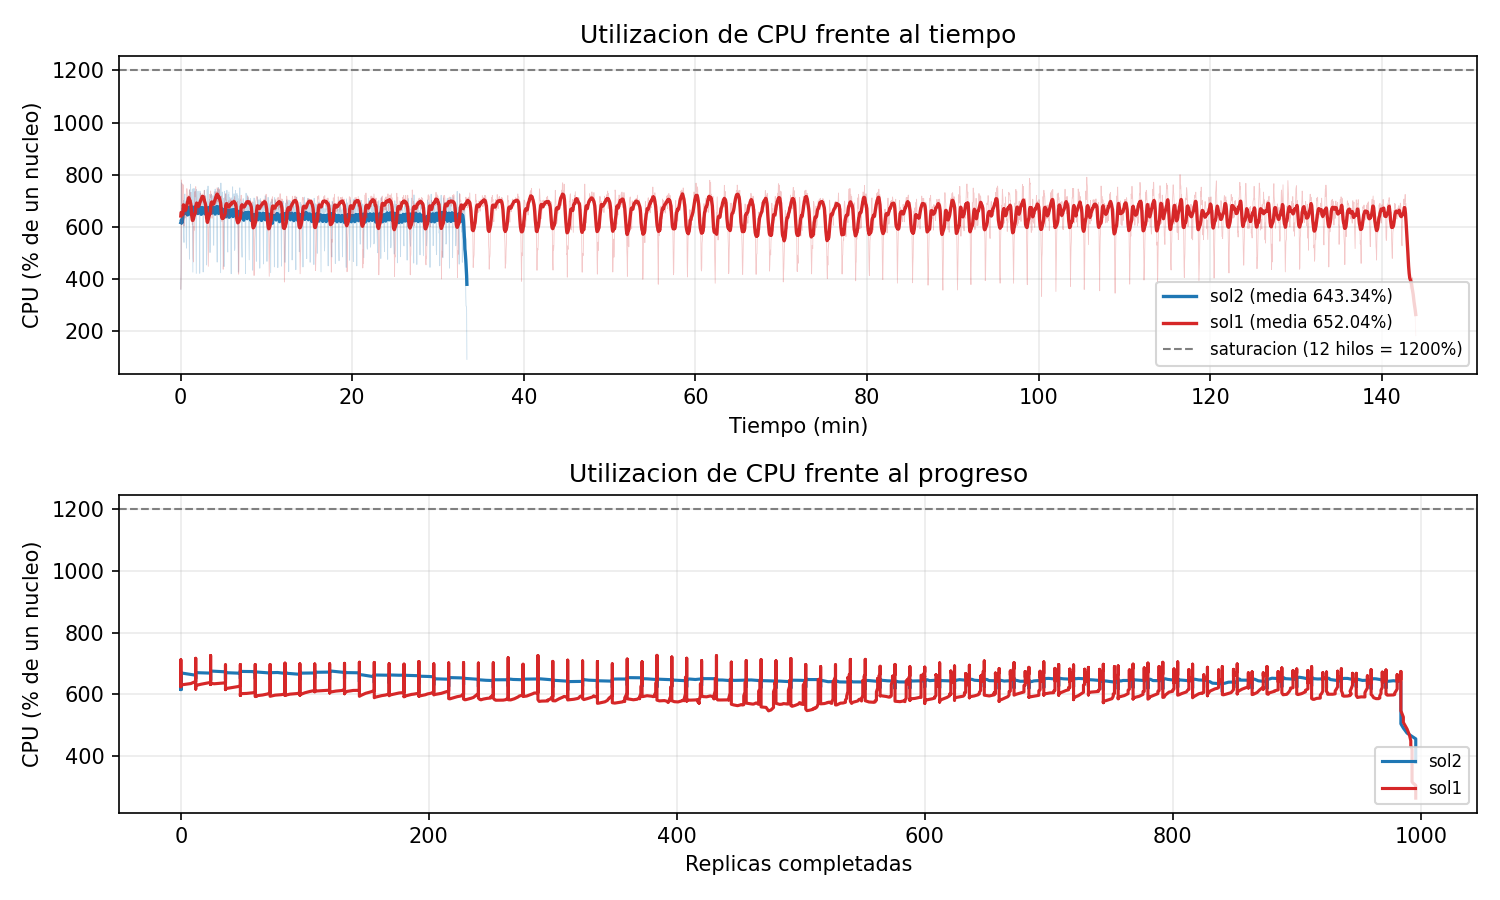
\includegraphics[trim=20 15 15 10, clip, width=\linewidth]{images/cmp_cpu.png}\\[0.3em]
  {\scriptsize\color{black!65}Utilización de CPU frente al tiempo}
\end{column}
\begin{column}{0.40\textwidth}
  \vspace{0.3em}
  \begin{tikzpicture}
  \node[fill=uc3mblue, rounded corners=3pt, drop shadow={opacity=0.25},
        text width=4.4cm, inner sep=10pt, align=center] {%
    \color{white}\bfseries\large 4,32$\times$\\[0.3em]
    \color{white}\mdseries\scriptsize razón entre ventanas de ejecución};
  \end{tikzpicture}

  \vspace{1em}
  {\scriptsize
  \textbf{\color{uc3mblue}Descartado}\\[0.5em]
  \textbullet\ \ Energía, potencia y temperatura\\[0.4em]
  \textbullet\ \ Recolección de basura (0,95\,\%)\\[0.4em]
  \textbullet\ \ Saturación de hilos\\[0.9em]
  \textbf{\color{uc3mblue}Origen}\\[0.5em]
  Ciclo de vida de los agentes pasajero y mensajería de los protocolos.}
\end{column}
\end{columns}

\vspace{0.5em}
\centering
{\scriptsize\color{black!65}Misma intensidad de cómputo, mayor duración.}
\end{frame}

% ======================================================================
\section{Conclusiones}
\begin{frame}[plain,noframenumbering]\sectionpage\end{frame}

\begin{frame}[t]{Conclusiones}
\vfill
\centering
\begin{tikzpicture}[
  sec/.style={draw=uc3mblue, line width=0.9pt, rounded corners=3pt,
              text width=3.2cm, minimum height=2.0cm, inner sep=8pt,
              align=center, font=\scriptsize}]

  \node[sec] (b) at (0,0) {\textbf{Arquitecturas equivalentes}\\[0.4em]
        0,37 frente a 0,36 de error estándar};
  \node[sec, left=0.55cm of b]  (a) {\textbf{Datos caracterizados}\\[0.4em]
        Distribuciones ajustadas estadisticamente para ocupación, subidas y bajadas};
  \node[sec, right=0.55cm of b] (c) {\textbf{Herramienta entregada}\\[0.4em]
        ejecución y visualización de KPIs};

  \node[fill=uc3mblue, rounded corners=3pt, drop shadow={opacity=0.25},
        text width=10.4cm, inner sep=12pt, align=center,
        above=1.5cm of b] (main) {%
    \color{white}\small\bfseries El sistema reproduce la operativa de la línea
    en días laborables, con un sesgo caracterizado de 2 pasajeros y una
    sobredispersión de origen identificado.};

  \coordinate (m) at ($(main.south)!0.5!(b.north)$);
  \draw[uc3mblue, line width=0.8pt] (main.south) -- (m);
  \foreach \n in {a,b,c} \draw[uc3mblue, line width=0.8pt] (m) -| (\n.north);
\end{tikzpicture}
\vfill
\end{frame}

\begin{frame}[t]{Limitaciones y líneas futuras}
\vspace{0.9em}
\centering
{\scriptsize
\renewcommand{\arraystretch}{3}
\begin{tabular}{@{}>{\raggedright\arraybackslash}p{4.6cm} c
                  >{\raggedright\arraybackslash}p{5.6cm}@{}}
\toprule
\textbf{Limitación} & & \textbf{Línea futura} \\
\midrule
Bajadas muestreadas de forma independiente por parada &
$\longrightarrow$ &
Modelar el descenso como proporción de la ocupación a bordo \\
Ocho meses de datos, sin ciclo anual completo &
$\longrightarrow$ &
Ampliar la cobertura para separar la componente estacional \\
Plataforma híbrida entre compilado e interpretado &
$\longrightarrow$ &
Migrar el motor a un lenguaje compilado \\
\bottomrule
\end{tabular}}


\end{frame}

% ======================================================================
\begin{frame}[plain,noframenumbering]
\begin{tikzpicture}[remember picture, overlay]
\fill[color=uc3mblue] (current page.south west) rectangle (current page.north east);
\node[anchor=west] at ([xshift=0.6cm] current page.west)
     {\usebeamerfont{title}\color{white}Gracias por su atención};
\end{tikzpicture}
\end{frame}


\guardacuenta

\appendix
\setcounter{framenumber}{0}
\setbeamertemplate{footline}{%
\vspace{-2em}\hfill\color{uc3mblue}\Roman{framenumber}\hspace{1em}\vspace{0.5em}}
% ======================================================================

\begin{frame}{Distribuciones ajustadas y selección por AIC}
\end{frame}

\begin{frame}{Depuración de datos: efecto de la MAD}
\end{frame}

\begin{frame}{Fichas completas de los protocolos FIPA}
\end{frame}

\begin{frame}{Validación por parada}
\end{frame}

\begin{frame}{Análisis de descarte del sobrecoste}
\end{frame}

\begin{frame}{Tránsitos degenerados y suelo temporal}
\end{frame}

\begin{frame}{Entorno de ejecución y reproducibilidad}
\end{frame}

\begin{frame}{Planificación y presupuesto}
\end{frame}

\begin{frame}{Marco regulador y entorno socioeconómico}
\end{frame}

\end{document}